% !TEX program = xelatex
% Laer Klokken Escapades — a broadside. One tabloid sheet on what the klokkers did
% in the clock channel the week of 14 September 2026, where they are going on
% Saturday, and what the platform handed them along the way.
% Sibling of papers/new-urls-fall-2026/new-urls-fall-2026.tex (same recipe).
\documentclass[10pt]{article}
\usepackage[paperwidth=11in,paperheight=17in,top=0.55in,bottom=0.5in,left=0.6in,right=0.6in]{geometry}
\usepackage{fontspec}
\usepackage{xcolor}
\usepackage{graphicx}
\usepackage{tabularx}
\usepackage{booktabs}
\usepackage{array}
\usepackage{ragged2e}
\usepackage{microtype}
\usepackage{tikz}
\usetikzlibrary{positioning,arrows.meta}
\usepackage{hyperref}
\hypersetup{colorlinks=true,urlcolor=acblue,linkcolor=acdark,pdftitle={Laer Klokken Escapades, September 2026}}

\setmainfont{lmsans10-regular.otf}[
  BoldFont=lmsans10-bold.otf,
  ItalicFont=lmsans10-oblique.otf,
  BoldItalicFont=lmsans10-boldoblique.otf,
]
\setmonofont{lmmonolt10-regular.otf}[Scale=0.92,
  BoldFont=lmmonolt10-bold.otf,
  ItalicFont=lmmonolt10-oblique.otf,
]
% YWFT display face for the masthead only; its punctuation and æøå are unreliable.
\newfontfamily\acbold{ywft-processing-bold}[Path=../../system/public/type/webfonts/,Extension=.ttf]
\newcommand{\dsep}{{\normalfont\;\textperiodcentered\;}}

\definecolor{acpink}{HTML}{B44887}
\definecolor{acpurple}{HTML}{7850B4}
\definecolor{acblue}{HTML}{1559A6}
\definecolor{acdark}{HTML}{312B38}
\definecolor{acgray}{HTML}{66636A}
\definecolor{acpale}{HTML}{F4F1F5}
\definecolor{acrule}{HTML}{DCD6DF}
\definecolor{acgreen}{HTML}{2D7650}
\definecolor{acorange}{HTML}{A85D24}
\newcommand{\acdot}{{\color{acpink}.}}
\newcommand{\ac}{Aesthetic{\acdot}Computer}

\pagestyle{empty}
\setlength{\parindent}{0pt}
\setlength{\parskip}{0pt}
\hyphenpenalty=10000\exhyphenpenalty=10000

% \host{favicon or empty}{name}{what it is}
\newcommand{\host}[3]{%
  \vspace{0.5em}%
  {\color{acdark}\rule{\linewidth}{1.6pt}}\par\vspace{0.3em}%
  {\ifx\relax#1\relax\else\raisebox{-0.22em}{\includegraphics[width=1.15em,height=1.15em]{figures/favicons/#1}}\ \fi{\ttfamily\bfseries\fontsize{12.5pt}{14pt}\selectfont\color{acdark}#2}}\par\vspace{0.1em}
  {\fontsize{8.6pt}{10.4pt}\selectfont\color{acgray}\RaggedRight#3\par}\vspace{0.6em}}
% \item: \addr{label}{headline}{body}{when}{who}{pill}
\newcommand{\addr}[6]{%
  \par\nointerlineskip{\color{acrule}\hrule height 0.5pt}\vspace{0.42em}%
  {\ttfamily\fontsize{9.3pt}{11pt}\selectfont{\bfseries\color{acpink}#1}\ {\bfseries\color{acdark}#2}}\par\vspace{0.16em}%
  {\fontsize{9.7pt}{12pt}\selectfont\color{acdark}\RaggedRight#3\par}\vspace{0.2em}%
  {\ttfamily\fontsize{7.2pt}{8.4pt}\selectfont\color{acgray}#4\ \ #5}\hfill#6\par\vspace{0.7em}}
\newcommand{\pill}[2]{{\fontsize{6.2pt}{7pt}\selectfont\colorbox{#1!12}{\textcolor{#1}{\bfseries\textls[60]{#2}}}}}
\newcommand{\shipped}{\pill{acgreen}{SHIPPED}}
\newcommand{\open}{\pill{acorange}{OPEN ASK}}
\newcommand{\saturday}{\pill{acpink}{SATURDAY}}
\newcommand{\hd}[1]{{\ttfamily\bfseries\fontsize{9.6pt}{11pt}\selectfont\color{acdark}#1}}
\newcommand{\dk}[1]{{\itshape #1}}
% \changed{who}{ask}
\newcommand{\changed}[2]{\par\nointerlineskip{\color{acrule}\hrule height 0.5pt}\vspace{0.4em}{\fontsize{9.4pt}{11.4pt}\selectfont\RaggedRight{\ttfamily\bfseries\color{acdark}#1}\ \ \color{acdark}#2\par}\vspace{0.45em}}

\begin{document}

% ═══════════════════════════════════════ masthead
{\ttfamily\fontsize{8.4pt}{10pt}\selectfont\color{acpink}\textls[80]{BROADSIDE\dsep LAER-KLOKKEN\dsep THE WEEK OF 14 SEPTEMBER 2026}\par}
\vspace{0.3em}
{\acbold\fontsize{50pt}{48pt}\selectfont\color{acdark}Laer Klokken\ \ {\color{acpink}Escapades}\par}
\vspace{0.55em}
\begin{minipage}[t]{0.63\linewidth}\vspace{0pt}
{\fontsize{11.4pt}{14.2pt}\selectfont\color{acdark}\RaggedRight
what the klokkers got up to in the clock channel this week, where they're all going on saturday, and what \ac{} handed them on the way. i read it off the chat and the git log on tuesday the 15th.\par}
\vspace{0.45em}
{\fontsize{8.2pt}{10pt}\selectfont\color{acgray}\href{https://prompt.ac/@jeffrey}{\color{acblue}\textbf{@jeffrey}}\ \textperiodcentered\ \ac{}\ \textperiodcentered\ laklok.com\ \textperiodcentered\ chat-clock\par}
\end{minipage}%
\hfill
\begin{minipage}[t]{0.33\linewidth}\vspace{0pt}
\renewcommand{\arraystretch}{0.9}
\begin{tabularx}{\linewidth}{@{}>{\raggedleft\arraybackslash}X>{\raggedleft\arraybackslash}X>{\raggedleft\arraybackslash}X@{}}
{\bfseries\fontsize{26pt}{26pt}\selectfont\color{acdark}100} & {\bfseries\fontsize{26pt}{26pt}\selectfont\color{acdark}11} & {\bfseries\fontsize{26pt}{26pt}\selectfont\color{acpink}4}\\
{\ttfamily\fontsize{6.6pt}{8pt}\selectfont\color{acgray}MSGS / DAY} & {\ttfamily\fontsize{6.6pt}{8pt}\selectfont\color{acgray}VOICES IN 24 H} & {\ttfamily\fontsize{6.6pt}{8pt}\selectfont\color{acgray}DAYS TO SHOWTIME}\\[0.5em]
{\bfseries\fontsize{26pt}{26pt}\selectfont\color{acdark}6} & {\bfseries\fontsize{26pt}{26pt}\selectfont\color{acdark}7} & {\bfseries\fontsize{26pt}{26pt}\selectfont\color{acdark}0}\\
{\ttfamily\fontsize{6.6pt}{8pt}\selectfont\color{acgray}GOING SO FAR} & {\ttfamily\fontsize{6.6pt}{8pt}\selectfont\color{acgray}CODES DROPPED} & {\ttfamily\fontsize{6.6pt}{8pt}\selectfont\color{acgray}LETTERS FROM OUTSIDE}\\
\end{tabularx}
\end{minipage}\par
\vspace{0.45em}
{\color{acdark}\rule{\linewidth}{3pt}}\par
\vspace{0.1em}

% ═══════════════════════════════════════ three columns
\begin{minipage}[t]{0.315\linewidth}\vspace{0pt}

\host{}{the trip}{folkets folkemøde, stubbekøbing, falster. a people's meeting without lobbyists --- talks, workshops, a market, one saturday a year. this year it has a clock in it.}
\addr{SAT 19}{laer klokken med goodiepal}{13:30 to 14:30 at rådhuset --- the town hall --- and it's in the printed program. their blurb: the composer and clockmaker records a new episode of his unpredictable radio show, about quitting social media for good and building your own computing on \ac{}. visitors are told to try the commands and catch up on old episodes. that's our pitch, written by someone else. the best kind.}{folketsfolkemøde.dk/program}{}{\saturday}
\addr{TUE 09:08}{the plan, seven points}{01 record a laer klokken program live. 02 every klokker in the room gets a segment. 03 the show runs 56 minutes. 04 there is no money, because there just isn't any. 05 a reception on the HVAD record. 06 a bed in stubbekøbing the night before and after. 07 a bus down from copenhagen --- if people say they're coming. coda: \dk{det bliver super duper}. it will.}{chat-clock}{@prutti}{}
\addr{WHO'S IN}{six so far, two asking about the bus}{@HendeFraHoeve first (\dk{jeg skal med!}), then @snakes, @YouthOrgan, @tyttebaer --- and @oliverstilling, who said back in august he'd see goodie there. @alki wants \dk{bus intel}. @osamakimlarsen wants to meet up beforehand \dk{og se hvem er folket}. @chigichigi asked when; the answer was the program link. prutti's reply to each of them: \dk{tjek}.}{2026-08-26 to 09-15}{}{}
\addr{LOGISTICS}{norway to copenhagen on friday}{prutti comes down friday. the festival sells its own bus tickets from copenhagen; prutti's bus needs a headcount. a bed in stubbekøbing is on offer the night before and after. no fee. no budget. no problem, apparently.}{}{}{}
\addr{TUE 10:15}{the phone line}{\dk{ring til Torras telefon. nu.} then \dk{linjen er åben nu} at 10:58, and again at 11:39. @tyttebaer and @YouthOrgan called in while the rest of the channel watched. the clock program is being made live, over a phone, in public, on a tuesday morning. that's the format.}{chat-clock}{@prutti @tyttebaer @YouthOrgan}{}

\end{minipage}%
\hfill{\color{acrule}\vrule width 1pt}\hfill
\begin{minipage}[t]{0.315\linewidth}\vspace{0pt}

\host{youtube.com.png}{the scene}{chat-clock, monday afternoon to tuesday afternoon --- about a hundred messages from eleven handles. danish and norwegian, english for the visitors.}
\addr{MON}{the chat became a video}{@FM\_Vigil recorded the chat and put it on youtube. @HendeFraHoeve cut it three times in one afternoon, chasing bigger text --- \dk{der kommer straks en version med større chat}, then \dk{større men mere uklar}, then \dk{alle gode gange 3}. prutti watched on an ipad at glasmagasinet in oslo: \dk{chatten er lidt lille men den er fucking fed}. the room is editing itself now. i just have to keep it running.}{2026-09-14}{@FM\_Vigil @HendeFraHoeve @prutti}{}
\addr{ALL WEEK}{codes on the wire}{kidlisp codes dropped bare into the channel, as art: \texttt{\#swk} from prutti; \texttt{\#w5o}, \texttt{\#n5j}, \texttt{\#v5x}, \texttt{\#ie6}, \texttt{\#6x3} from @osamakimlarsen (\dk{\#ie6 har til gengæld lavet programmet en del mere indbringende}); \texttt{\#aue} from @q13R608tx --- \dk{süper sygnok}. earlier in the month \texttt{\#jzg} and \texttt{\#4ne} did the rounds in the front room too. three characters, no preview, click it and see. that was the whole idea.}{2026-08-21 to 09-15}{}{}
\addr{MON EVE}{datamusik provenance}{@q13R608tx and @snakes spent the evening on who really made the datamusik records and the V/Vm audio --- ``jansky noise has also confirmed that datamusik 13 and 03 are both made by you.'' snakes: he made more sounds than he remembers. q13 is \dk{soldering a bunch of wires once more to create a product}, and thanked osama for the stickers and the collage. the archive argues with itself. good.}{2026-09-14}{}{}
\addr{MON}{r8dio housekeeping}{@Wallowing asked whether the roskilde concert came down from r8dio over music rights. prutti: no --- programs get deleted \dk{efter forgodtbefindende}, at whim. @FM\_Vigil had been \dk{helt ude af AC, det har drillet meget}; @HendeFraHoeve agreed it's been \dk{lidt ustabil på det seneste}. that one's mine to fix, not theirs.}{2026-09-14}{}{\open}
\addr{SINCE AUG}{the main chat is a signpost}{nearly every message in /chat since mid-august tells a newcomer to click the blue text: \dk{vi har gang i} `laer-klokken'. @Gumpen, @ildispose, @iltis, @QualBornholmo, @darsh.tv and @vec all came in that way. the front room exists to point at the back room. fine by me.}{chat-system}{}{}

\end{minipage}%
\hfill{\color{acrule}\vrule width 1pt}\hfill
\begin{minipage}[t]{0.315\linewidth}\vspace{0pt}

\host{aesthetic.computer.png}{what the platform handed them}{everything here landed in the last thirty days. most of it i built for this room.}
\addr{09-13}{two laklok sisters, one census}{the raster laklok piece and the vector laklok.com/html now stay in lockstep, and both report which tema each visitor wears. a \texttt{realtime} tema drifts with the calendar. edit one sister, edit the other --- or they drift.}{b7037992a4}{laklok:nat:links}{\shipped}
\addr{09-08}{prutti's words learned to speak}{a vox chip on every @prutti message --- his consented elevenlabs voice reads the line back with per-word karaoke timing. since 09-13 any signed-in handle can send a text through \texttt{say}.}{648e73a46e}{pruttivox}{\shipped}
\addr{09-01}{laer-klokken TV, and the bridge back}{a 24/7 youtube stream of the clock room, with a chat bridge that seats youtube live-chat viewers in chat-clock as televised guests. this is the rig @FM\_Vigil's recording came off. the television watches the chat; the chat watches the television.}{c894adb754}{tvchat}{\shipped}
\addr{09-13}{every klokker is an email address}{\texttt{prutti@aesthetic.computer} exists. the door is open, SPF and DKIM are on, and nobody has told the room. prutti asked on 09-08 where to send three files ``for computer change'' and again on 09-11 --- \dk{what email adress should i use to file things to you?} letters from outside so far: zero. @q13R608tx worked it out on his own: ``mail is the new private messaging system basically... but even better because its mail!!'' he's right. i should say so.}{f6be8556c6}{amail}{\open}
\addr{09-04}{goodiepal cannot log in}{@snakes relayed it in the front room: \dk{message in laklpk goodiepal can not log in}. nothing in the chat says it got solved. the auth0 email-identity merge landed 09-11 --- worth checking whether that was the cure, before saturday. the host of the show should be able to get into his own show.}{chat-system}{@snakes}{\open}
\addr{09-12}{the ui says i have to verify a AC..?}{@kitten.cat hit the verify prompt and didn't know what it wanted. that's copy, not code. one sentence would fix it.}{chat-system}{@kitten.cat}{\open}

\end{minipage}\par

% ═══════════════════════════════════════ the week (diagram)
\vspace{0.6em}
{\color{acdark}\rule{\linewidth}{1.6pt}}\par\vspace{0.35em}
{\ttfamily\fontsize{8pt}{9.5pt}\selectfont\color{acpink}\textls[80]{THE ROAD TO STUBBEKØBING}\par}
\vspace{0.1em}
\begin{center}
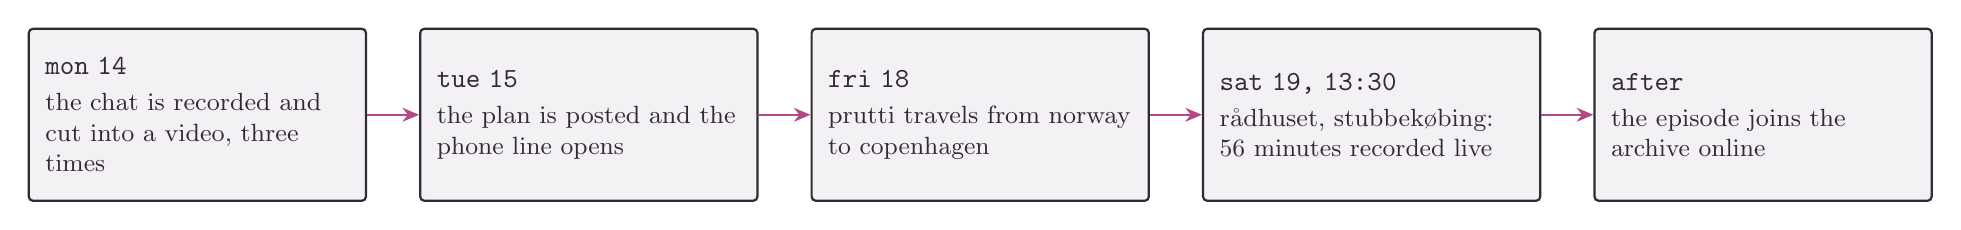
\begin{tikzpicture}[
  node distance=0.26in,
  box/.style={draw=acdark, line width=0.8pt, rounded corners=1.5pt, fill=acpale, text width=1.52in, minimum height=0.86in, align=left, inner sep=6pt, font=\fontsize{9.2pt}{11pt}\selectfont\color{acdark}},
  arr/.style={-{Stealth[length=6pt,width=5pt]}, line width=0.9pt, draw=acpink}
]
\node[box] (a) {\hd{mon 14}\\[2pt]the chat is recorded and cut into a video, three times};
\node[box, right=of a] (b) {\hd{tue 15}\\[2pt]the plan is posted and the phone line opens};
\node[box, right=of b] (c) {\hd{fri 18}\\[2pt]prutti travels from norway to copenhagen};
\node[box, right=of c] (d) {\hd{sat 19, 13:30}\\[2pt]rådhuset, stubbekøbing: 56 minutes recorded live};
\node[box, right=of d] (e) {\hd{after}\\[2pt]the episode joins the archive online};
\draw[arr] (a) -- (b); \draw[arr] (b) -- (c); \draw[arr] (c) -- (d); \draw[arr] (d) -- (e);
\end{tikzpicture}
\end{center}
\vspace{0.3em}

% ═══════════════════════════════════════ footer
{\color{acdark}\rule{\linewidth}{3pt}}\par\vspace{0.45em}
\begin{minipage}[t]{0.63\linewidth}\vspace{0pt}
{\ttfamily\fontsize{8pt}{9.5pt}\selectfont\color{acpink}\textls[80]{IF I ANSWER FOUR THINGS IN CHAT THIS WEEK}\par}\vspace{0.35em}
\begin{minipage}[t]{0.48\linewidth}\vspace{0pt}
\changed{@prutti}{tell him his address is prutti@aesthetic.computer, and the three files can go there. first real letter through the door.}
\changed{@snakes / goodiepal}{ask whether the login still fails after the 09-11 identity merge. if it does, it's the one thing that could keep saturday's host off his own platform.}
\end{minipage}\hfill
\begin{minipage}[t]{0.48\linewidth}\vspace{0pt}
\changed{@kitten.cat}{say in one line what ``verify'' means, then fix the copy so nobody has to ask again.}
\changed{@HendeFraHoeve}{a bigger-chat tema for the video cuts would save her the third re-render next time. she's already doing the work --- give her the knob.}
\end{minipage}
\end{minipage}\hfill
\begin{minipage}[t]{0.33\linewidth}\vspace{0pt}
{\ttfamily\fontsize{7.6pt}{9pt}\selectfont\color{acpink}\textls[80]{HOW TO READ THIS}\par}\vspace{0.3em}
{\fontsize{8.4pt}{10.2pt}\selectfont\color{acgray}\RaggedRight
quotes are from the AC chat channels \texttt{chat-system} and \texttt{chat-clock}, read on 2026-09-15. danish and norwegian are left as written, in italics. handles are the public AC handles the messages were posted under. counts are the last 100 messages in chat-clock, 09-14 13:37 to 09-15 14:47. program details are from folketsfolkemøde.dk. platform items cite the commit that shipped them.\par
\vspace{0.4em}
icons are the ones each host serves: the AC mark for laklok.com and the platform column, youtube's for the scene column. folketsfolkemøde.dk serves no favicon, so the trip column goes without. set in YWFT Processing, Latin Modern Sans and Latin Modern Mono. \ac{}\par}
\end{minipage}

\end{document}
